Ordini la spesa online e ti arriva a casa in un'ora.
Supermercato24 è la \textit{Start-Up} che mette in contatto chi vuole acquistare prodotti online dai supermercati e i \textit{``personal shopper''}, persone che fanno la spesa per conto del cliente e la consegnano a domicilio.
Nata a Verona nel settembre 2014 da un'idea di Enrico Pandian, oggi conta 30 dipendenti e più di settecento fattorini dislocati nelle 16 province italiane servite.
Utilizzare il servizio di Supermercato24 è piuttosto semplice, basta inserire il proprio codice di avviamento postale sul sito.
A quel punto il portale elenca i supermercati convenzionati più vicini.
Una volta selezionati i prodotti e inviato l'ordine, un fattorino che lavora con Supermercato24 fa la spesa al posto del cliente e la consegna entro un'ora \cite{Supermercato24}.

Il modello di business si basa su tre fattori: costo di consegna della spesa (4.90 \euro{}), accordi con le grandi marche e sovrapprezzo sul prodotto acquistato.
Il mercato del \textit{grocery} in Italia vale circa 180 miliardi, ma è attivo per lo più offline, con un'incidenza potenziale legata all'e-commerce dell'1\%.
Una fetta da oltre un miliardo e mezzo di euro, che potrebbe far gola a tanti \cite{Pitch}.

Supermercato24 è attiva in 16 province e 300 comuni, esegue circa 500 consegne al giorno e serve tramite i suoi \textit{``shopper''} oltre 40mila clienti, facendo leva su più di 30 insegne.
In catalogo ha circa 90mila articoli, il tasso di crescita mese su mese è del 15\% (a giugno le consegne hanno toccato quota 300mila), ha attualmente 250mila utenti e ha chiuso il 2016 con un fatturato di circa 6 milioni di euro, a fronte dei 750mila del 2015 \cite{Aucap}.

Nel 2016 è stato siglato un accordo tra Supermercato24 e Samsung, per portare il portale e-commerce all'interno della linea frighi smart \verb+IoT+ dell'azienda sudcoreana.
La soluzione si chiama Samsung Family Hub e unisce domotica e commercio elettronico, ed è stato presentato all'IFA di Berlino a Settembre \cite{Samsung}.
Attraverso uno schermo esterno, incorporato nell'anta del frigo, è possibile ordinare la spesa con il proprio account.
Nel futuro sarà possibile comprare i prodotti, non appena esauriti, attraverso telecamere e sensori interni.

\begin{figure}[H]
  \centering
  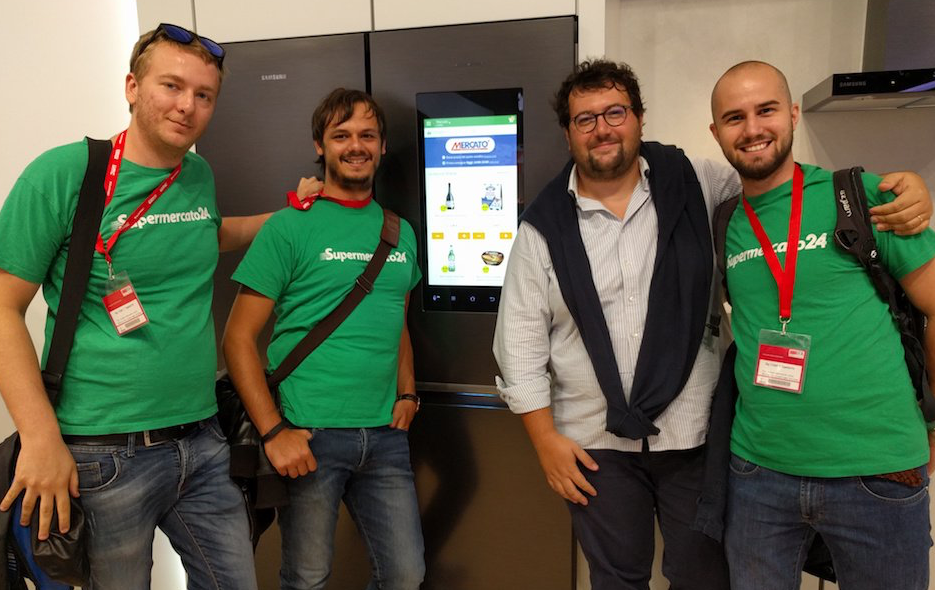
\includegraphics[width=0.95\linewidth, keepaspectratio]{samsung}
  \caption{Presentazione della linea Samsung Family Hub all'IFA del Settembre 2016}
  \label{fig:samsung}
\end{figure}

\subsection{Panoramica tecnica}
\label{subsec:supermercato24Panoramica}

La piattaforma di Supermercato24 è costituita da due Applicativi monolitici scritti in \verb+Php 5.5+ con il framework \textit{Laravel}.
Otto Microservizi gestiscono le varie integrazioni e namespace.
Il Database utilizzato è \verb+MySQL 5.6+ in \textit{cluster} su due \textit{server} in \textit{High Availability} che si occupa di gestire catalogo/utenze/negozi/ordini.
Viene utilizzato il KeyValue \verb+Redis 2.8+ per gestire: i \textit{token} di sessione degli utenti, i carrelli non ancora confermati e i messaggi asincroni.
I Client sono scritti in: \verb+Javascript+ con il framework \textit{Angular} per la parte \textit{browser}, \verb+Java+ per la parte \textit{Android} e \verb+Objective-C+ per la parte \textit{iOS}.
È disponibile un ambiente di \textit{staging} per controllare il corretto funzionamento della piattaforma avvalorato da \textit{UnitTest}.

Per il lavoro della tesi è stato utilizzato \verb+RaspberryPi 3+ come \textit{server} stand-alone e \verb+NodeJs 7+ come \textit{back-end} che si occupa della gestione delle connessioni dei \textit{socket}.
Nelle prossime sezioni entrerò nel dettaglio dell'architettura appena descritta, evidenziando i problemi emersi e le soluzioni adottate.

\subsection{Struttura del Sistema}
\label{subsec:supermercato24StrutturaSistema}

Supermercato24 si compone di diversi componenti suddivisi con scopi specifici, i quali dialogano, se previsto, tramite \verb+API KEY+ o \verb+WebHook+.
il progetto \textit{Sm} si occupa di fornire diverse \verb+API+ a tutti i \textit{client} per sfogliare il catalogo dell'e-commerce.
La comunicazione è fatta tramite chiamate \verb+HTTP+ e nel lavoro di tesi si cercherà di sincronizzarla in tempo reale (evidenziata in rosso nella figura \ref{fig:s24_system}).
I clienti posso usufruire del servizio con il proprio browser o utilizzare la relativa app e sono accreditati dal progetto \textit{User} tramite \textit{token} di sessione salvato nel KeyValue.
I prodotti sono catalogati per mezzo del progetto \textit{Cp24}, il quale fornisce un backoffice agli operatori e lavora in maniera sinergica con il progetto \textit{Gdo} per aggiornare i prezzi raccolti da repository esterni.
Ad ogni ordine creato c'è uno scambio di informazioni verso il progetto \textit{S24}, il quale fa transitare l'ordine al fattorino migliore e offre un backoffice di controllo ai relativi responsabili.
I fattorini si abilitano nella piattaforma con il progetto \textit{Community} e ricevono comunicazioni tramite il progetto \textit{Sms}.
Ogni fattorino può chiamare il proprio cliente tramite il progetto \textit{Phdlv} che si frappone come proxy telefonico tra lo shopper e il cliente.
Infine il progetto \textit{DataAnalyst} confronta i Database dei vari progetti per estrarre metriche e analisi  di business.

\begin{figure}[H]
  \centering
  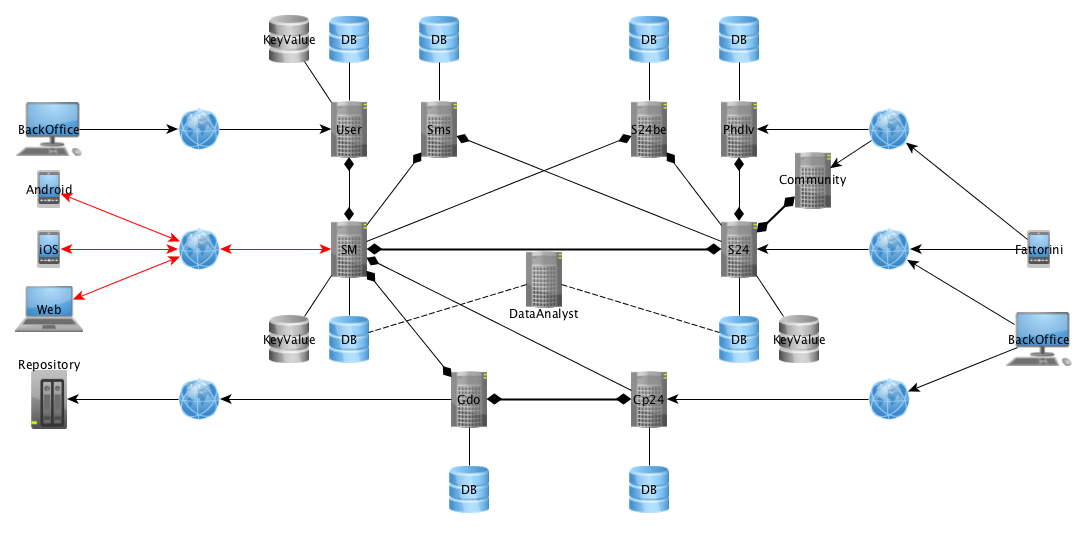
\includegraphics[angle=90, width=11.5cm, keepaspectratio]{s24}
  \caption{Modello della struttura di Supermercato24}
  \label{fig:s24_system}
\end{figure}

\subsection{Struttura del Database}
\label{subsec:supermercato24StrutturaDatabase}

I prodotti all'interno dell'e-commerce sono organizzati secondo una relazione binaria \verb+N:N+ tra la tabella \textit{Item} e la tabella \textit{Store}.
La tabella \textit{Item} contiene tutti i dettagli di un prodotto quali nome, marchio, EAN, immagini e grammatura.
Ogni prodotto può essere salvato nella tabella \textit{Bookmark} come preferito da parte del cliente.
Tutti i prodotti sono catalogati attraverso una categoria di terzo livello univoca (foglia) tramite una relazione \verb+N:1+.
La tabella \textit{Category} contiene un'alberatura ricorsiva di elementi collegati tra di loro, per definire una struttura a livelli sovrapposti.

La tabella \textit{Store} contiene tutti i dettagli dei negozi disponibili nella piattaforma.
Ogni negozio ha a disposizione i propri orari di apertura nella tabella \textit{StoreTime} tramite una relazione \verb+1:N+ e sono catalogati per insegna nella tabella \textit{StoreBrand} tramite una relazione \verb+N:1+.

Infine la tabella \textit{ItemStore} contiene i prezzi dei prodotti presenti in determinati supermercati, dove alcuni sono aggiornati quotidianamente tramite accordi commerciali con la GDO.

Quando un cliente effettua un ordine, lo stato di ogni prodotto viene salvato nella tabella \textit{OrderDetail} in relazione \verb+N:1+ con la tabella \textit{Order}.

La maggior parte delle tabelle del Database utilizzano il motore \verb+InnoDB+ per usufruire delle proprietà \verb+ACID+ tramite \textit{Foreign Key}.
La tipologia di \textit{locking}, a livello di riga, permette di aggiornare (in scrittura) il catalogo giornalmente senza causare disservizi ai clienti che stanno navigando sul sito (in lettura).

\begin{figure}[H]
  \centering
  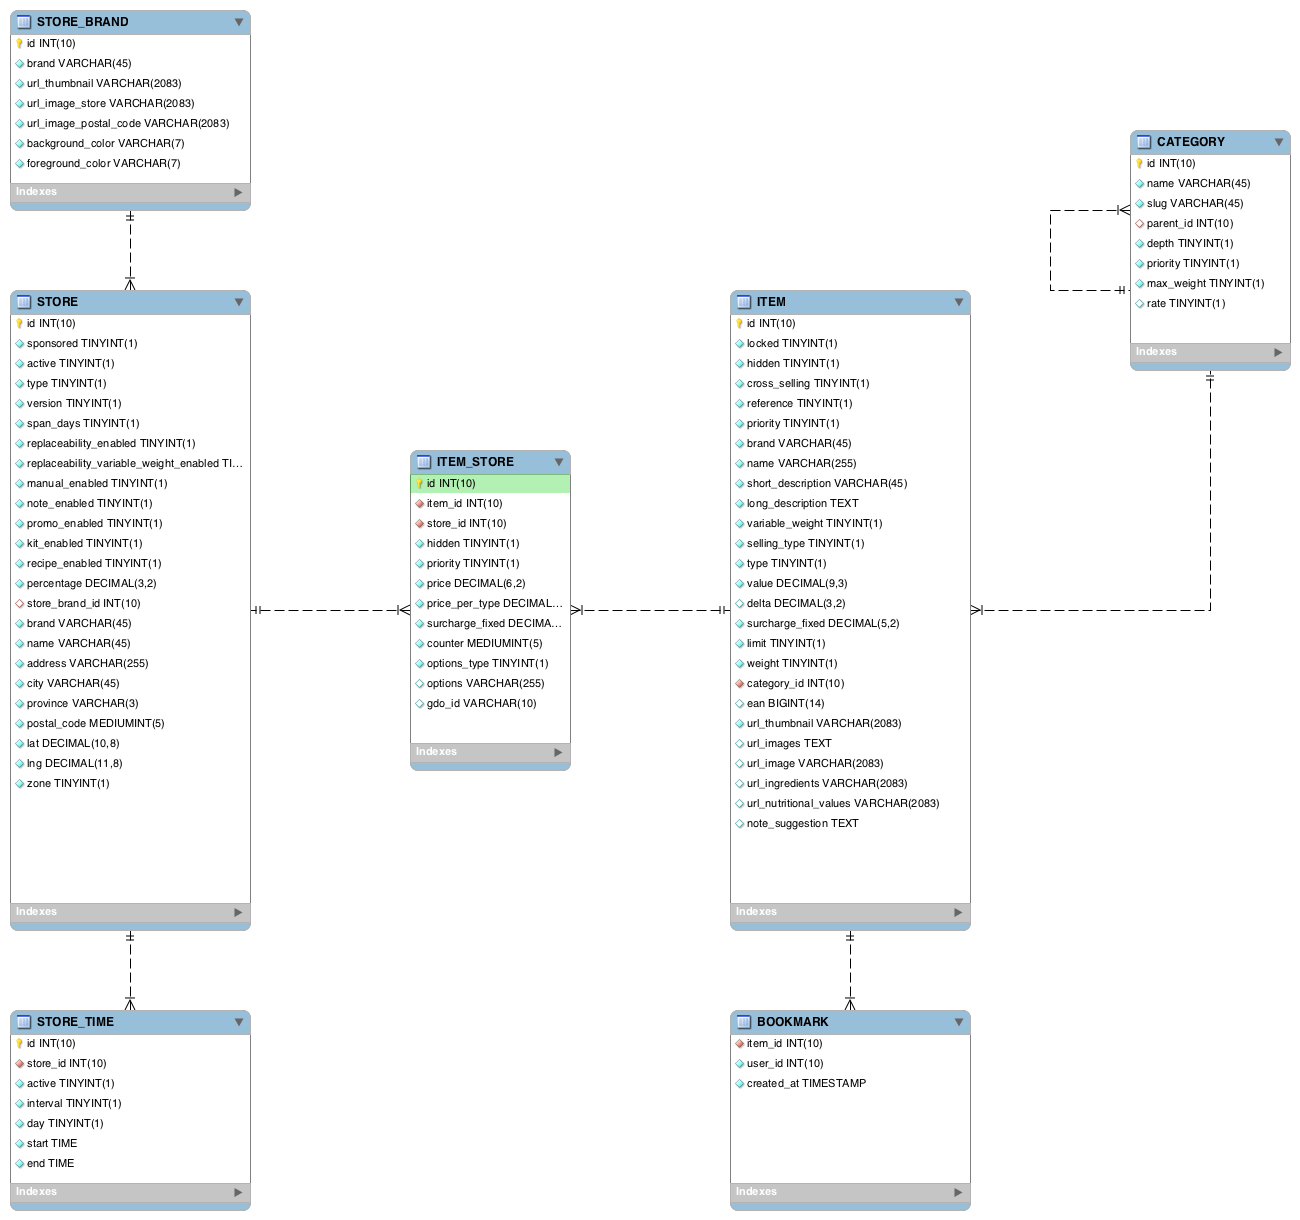
\includegraphics[width=0.95\linewidth, keepaspectratio]{sql_db}
  \caption{Modello E-R della struttura del Database}
  \label{fig:sql_db}
\end{figure}

Dato l'identificativo del negozio, sono necessarie sei \textit{Join} per ottenere tutti i dettagli di un prodotto, combinando le tuple delle relazioni appena definite e controllando tutti i rispettivi \textit{flag} di attivazione e ordinamento.

\begin{lstlisting}[language=sql, label={lst:supermercato24DatabaseBefore}, captionpos=b, caption={Query originaria per ottenere le informazioni di un prodotto}, basicstyle=\scriptsize\ttfamily]
SELECT *
FROM ITEM i
    JOIN ITEM_STORE ss ON ss.item_id = i.id AND ss.hidden = 0
    JOIN STORE s ON s.id = ss.store_id AND s.active = 1
    JOIN CATEGORY c3 ON c3.id = i.category_id AND c3.depth = 2
    JOIN CATEGORY c2 ON c2.id = c3.parent_id AND c2.depth = 1
    JOIN CATEGORY c1 ON c1.id = c2.parent_id AND c1.depth = 0
    LEFT JOIN BOOKMARK b ON b.item_id = i.id AND b.user_id = 32600
WHERE
    i.hidden = 0 AND ss.store_id = 5030;
\end{lstlisting}

\begin{figure}[H]
  \centering
  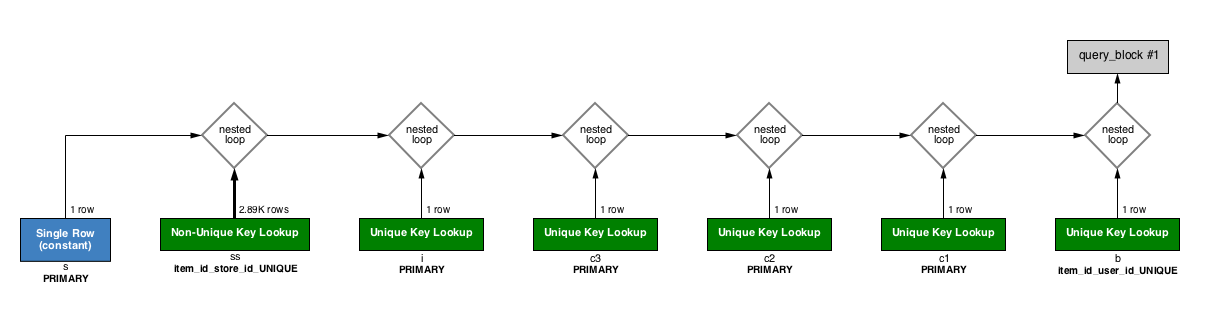
\includegraphics[width=0.95\linewidth, keepaspectratio]{sql_before}
  \caption{Execution Plan della query originaria per ottenere le informazioni di un prodotto}
  \label{fig:sql_before}
\end{figure}

Queste combinazioni sono state successivamente raccolte in una \textit{View} e raggruppate in una tabella temporanea volatile \verb+MEMORY+ compilata giornalmente ordinata con i rispettivi \textit{flag} di attivazione.

\begin{lstlisting}[language=sql, label={lst:supermercato24DatabaseAfter}, captionpos=b, caption={Query ottimizzata per ottenere le informazioni di un prodotto}, basicstyle=\scriptsize\ttfamily]
SELECT *
FROM PRODUCT p
    LEFT JOIN BOOKMARK b ON b.item_id = p.item_id AND b.user_id = 32600
WHERE
    store_id = 5030;
\end{lstlisting}

\begin{figure}[H]
  \centering
  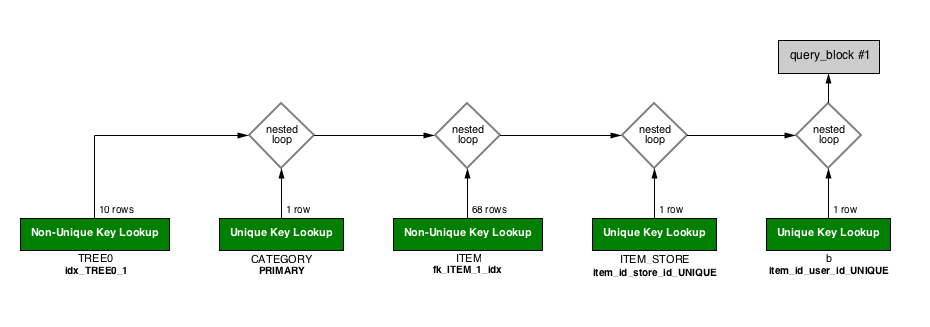
\includegraphics[width=0.95\linewidth, keepaspectratio]{sql_after}
  \caption{Execution Plan della query ottimizzata per ottenere le informazioni di un prodotto}
  \label{fig:sql_after}
\end{figure}

Come si evince dal confronto delle due immagini, la normalizzazione delle tabelle ha ridotto le relazioni necessarie per ottenere una o più risorse dal sistema.
Con il progetto della sezione \ref{sec:smiot} si cercherà di rendere questo modello accessibile in tempo reale.
A seguito di un determinato evento, come l'aggiunta di un preferito, la creazione di un ordine o l'aggiornamento del catalogo, sarà compito dell'applicativo propagare tali dati al giusto utente.

\subsection{Struttura dell'Architettura}
\label{subsec:supermercato24StrutturaArchitettura}

Tutte le risorse sono organizzate secondo l'architettura \verb+RESTful+, quindi consumabili con il metodo \verb+HTTP+ \verb+GET+ \cite{Rest}.

Il carrello è una risorsa salvata temporaneamente tramite KeyValue, secondo l'associazione \verb+N:N+ Negozio:Cliente con la struttura \verb+HASH+.
Questa associazione fornisce la chiave necessaria per accedere al carrello, il cui valore è la quantità del prodotto scelta dal cliente.

\begin{lstlisting}[language=bash, label={lst:supermercato24Architettura}, captionpos=b, caption={Elenco dell'operazioni effettuate nel carrello da parte del cliente}, basicstyle=\scriptsize\ttfamily]
redis> HSET store_id_user_id item_store_id 1.2
(integer) 1
redis> HGET store_id_user_id item_store_id
"1.2"
redis> HINCRBYFLOAT store_id_user_id item_store_id 0.4
"1.6"
redis> HINCRBYFLOAT store_id_user_id item_store_id -0.6
"1"
redis> HDEL store_id_user_id item_store_id
(integer) 1
redis> HGET store_id_user_id item_store_id
(nil)
\end{lstlisting}

Ogni modifica della quantità di un prodotto avviene tramite metodo \verb+HTTP+ \verb+PUT+, mentre l'eliminazione tramite metodo \verb+HTTP+ \verb+DELETE+.
Ogni azione ha una complessità temporale $O(1)$.

Quando il cliente ha completato il proprio carrello, risulterà possibile effettuare l'ordine tramite metodo \verb+HTTP+ \verb+POST+.
Salvati l'indirizzo di spedizione, l'orario di consegna e il metodo di pagamento appropriato questi dati vengono recapitati al fattorino migliore.
Con il progetto della sezione \ref{sec:socksberry} si cercherà di notificare in tempo reale la creazione di un ordine tramite \textit{dashboard}.
Queste informazioni serviranno per avvertire gli operatori e misurare l'efficienza del servizio.
